\section{Bidirectional Mapping mechanism}
\label{sec:mappingmechanism}
In this section, we describe the mapping mechanism, which consists of a bidirectional mapping (see \ref{subsec:bimapping}) and a text-to-text transformation (see \ref{subsec:compilation}).

\subsection{Bidirectional mapping through an example}
\label{subsec:bimapping}
We present here our bidirectional mapping between UML-based architecture models and code through a producer-consumer example, whose architecture is specified by Fig. \ref{fig:approachexample} \encircle{a}, \encircle{b}, and \encircle{c}.
The \ttt{p} producer sends data items to a first-in first-out component \ttt{FIFO} storing data.
The \ti{FIFO} queue has a limited size, the number of currently stored items (\ttt{numberOfItems}) and the \ttt{isQueueFull} operation for validating its availability.
The \ti{pPush} port of the producer with \ttt{IPush} as required interface is connected to the \ti{pPush} port of \ti{FIFO} with \ttt{IPush} as provided interface. 
The producer and \ti{FIFO} can interact with each other through their respective port.
\ttt{FIFO} also provides the \ti{IPull} interface for the consumer to get data items.
\ti{FIFO} implements the two interfaces as in Fig. \ref{fig:approachexample} \encircle{b}, lines 28-29.

The behavior of \ttt{FIFO} is described by using a UML State Machine as shown in Fig. \ref{fig:approachexample} \encircle{c}.
Initially, the \ttt{Idle} state is active.
The state machine then waits for an item to arrive at the \ttt{fifo} component (through the \ttt{pPush} port).
The item is then checked for its validity before verifying the fullness of the queue to decide to either add to the queue or discard it.


Table \ref{table:mapping} and \ref{table:mapping2} show some of the UML meta-classes and our ad-hoc equivalent constructs in the extended language.
The constructs are categorized into \ti{structural} (four upper rows in Table \ref{table:mapping2} and \ref{table:mapping2}) and \ti{behavioral constructs} (nine lower rows in Table \ref{table:mapping2}).
We explain these constructs in the followings.

\begin{comment}
\begin{table}[]
	\centering
	\caption{My caption}
	\label{my-label}
	\begin{tabular}{lllll}
		UML                  & XGC                      &  & OO                             & C++                 \\ \cline{1-2} \cline{4-5} 
		Class component      & Class                    &  & Class                          & Class               \\ \cline{1-2} \cline{4-5} 
		Part                 & Part                     &  & Composition attribute          & Attribute           \\ \cline{1-2} \cline{4-5} 
		Port  (data/control) & Port                     &  & Attribute                      & Reference Attribute \\ \cline{1-2} \cline{4-5} 
		Many ports           & Multiple-port            &  & Multiple interface realization & --                  \\ \cline{1-2} \cline{4-5} 
		Connector            & Binding (static+dynamic) &  & --                             & Methods             \\ \cline{1-2} \cline{4-5} 
		Interface            & Class/Interface          &  & Interface                      & Class               \\ \cline{1-2} \cline{4-5} 
		Signal               & Class                    &  & Class                          & Class/Struct        \\ \cline{1-2} \cline{4-5} 
		State machine        & state\_machine           &  & --                             & --                  \\ \cline{1-2} \cline{4-5} 
		State                & state                    &  & --                             & --                  \\ \cline{1-2} \cline{4-5} 
		Region               & region                   &  & --                             & --                  \\ \cline{1-2} \cline{4-5} 
		CallEvent            & call\_event              &  & --                             & --                  \\ \cline{1-2} \cline{4-5} 
		TimeEvent            & time\_event              &  & --                             & --                  \\ \cline{1-2} \cline{4-5} 
		ChangeEvent          & change\_event            &  & --                             & --                  \\ \cline{1-2} \cline{4-5} 
		SignalEvent          & signal\_event            &  & --                             & --                  \\ \cline{1-2} \cline{4-5} 
		Any                  & any                      &  & --                             & --                  \\ \cline{1-2} \cline{4-5} 
		Pseudo state         & pseudo\_state            &  & --                             & --                  \\ \cline{1-2} \cline{4-5} 
		Action/Effect        & Method                   &  & Method                         & Method             
	\end{tabular}
\end{table}
\end{comment}

\begin{table}[]
	\centering
	\caption{Mapping between UML and Examples of Extended Language}
	\label{table:mapping}
	\begin{tabular}{lll}
		UML                                                                      & Extended Language                                                                                & Code example in Fig. \ref{fig:approachexample}                                                                               \\ \hline
		\begin{tabular}[c]{@{}l@{}}Port requiring \\ an interface \ti{I}\end{tabular} & \begin{tabular}[c]{@{}l@{}}Attribute typed \\ by \ti{RequiredPort}\textless I\textgreater\end{tabular} & \begin{tabular}[c]{@{}l@{}}Ports \ti{pPush} and \ti{pPull} at lines\\ 21 and 25\end{tabular}         \\ \hline
		\begin{tabular}[c]{@{}l@{}}Port providing \\ an interface \ti{I}\end{tabular} & \begin{tabular}[c]{@{}l@{}}Attribute typed\\ by \ti{ProvidedPort}\textless I\textgreater\end{tabular}  & \begin{tabular}[c]{@{}l@{}}Ports \ti{pPush} and \ti{pPull} at \\ lines 29-30\end{tabular}            \\ \hline
		Connector                                                                & Binding                                                                                        & Lines 7-8                                                                                  \\ \hline
		State Machine                                                            & \ti{StateMachine}                                                                                     & \begin{tabular}[c]{@{}l@{}}The FIFO state machine at \\ lines 34-59\end{tabular}           \\ \hline
		State                                                                    & \ti{State/InitialState}                                                                               & \begin{tabular}[c]{@{}l@{}}State \ti{SignalChecking} at \\ lines 36-39\end{tabular}             \\ \hline
		Region                                                                   & \ti{Region}                                                                                           & Not shown in this paper                                                                                 \\ \hline
		Pseudo state                                                             & \begin{tabular}[c]{@{}l@{}}Attribute typed \\ by pseudo type\end{tabular}                        & \begin{tabular}[c]{@{}l@{}}The \ti{dataChoice} pseudo state \\ at line 49\end{tabular}          \\ \hline
		Action/Effect                                                            & Method                                                                                           & Methods at lines 60-65       \\ \hline
		Transitions                                                           & Transition table                                                                                           & Transition table at lines 51-58	\\ \hline
		Event                                                            & Event                                                                                           & The call event at line 50                                                             
	\end{tabular}
\end{table}



\subsubsection{Structural constructs}
This section explains the programming constructs in the bidirectional mapping corresponding to the modeling concepts used for modeling the architecture structure, including \ti{Port} and \ti{Binding}.

%\noindent
%\tb{Part:}
%In the extended language, we introduce the \ti{Part<T>} template class.
%A UML part is typed by a UML class and mapped to a standard class attribute typing the template class with the \ti{T} template parameter replaced by the class equivalent to the UML class typing the UML part. 
%For example, at line 3, the \ti{p} attribute is equivalent to the \ti{p} part in the model.

\begin{figure*}
	\centering
	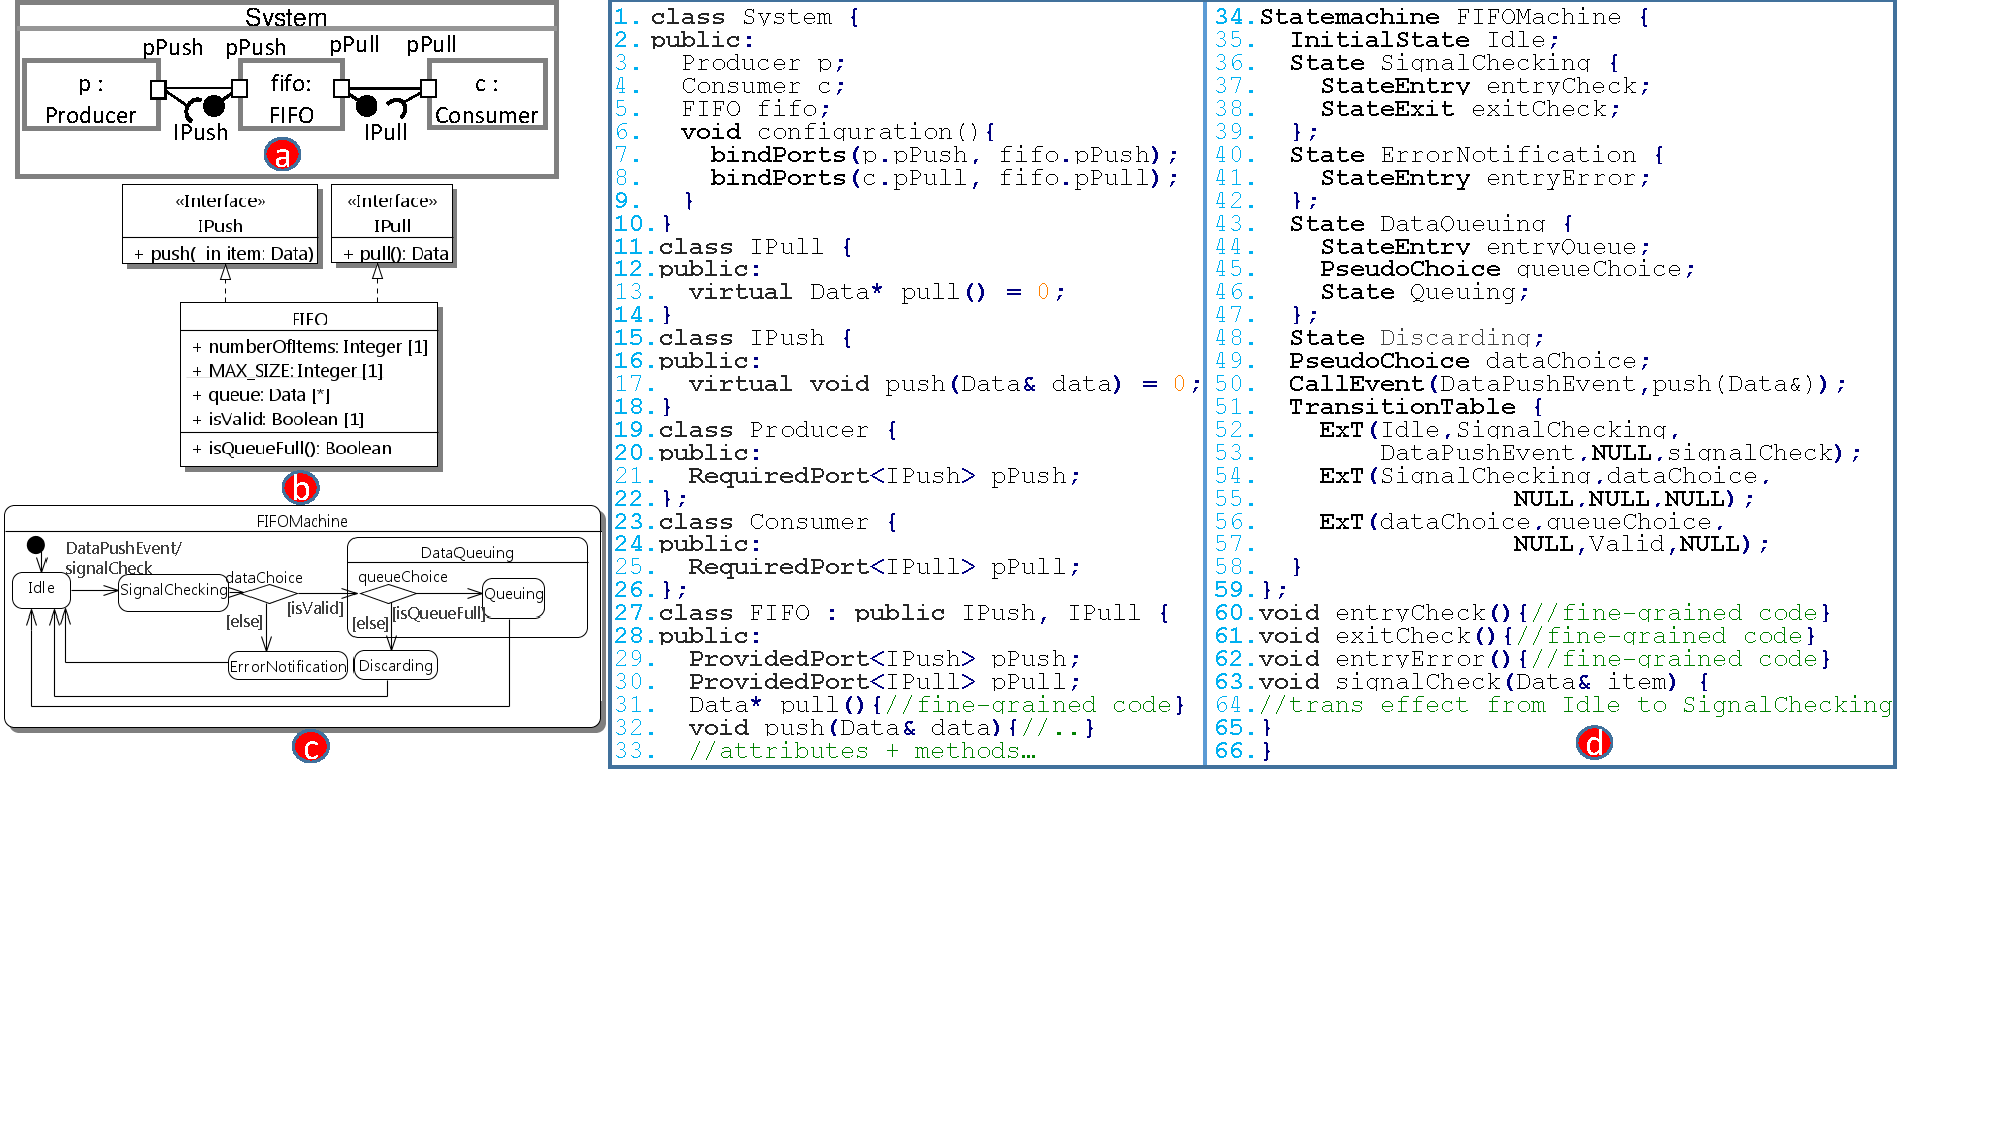
\includegraphics[clip, trim=0cm 7cm 1.0cm 0cm, width=\textwidth]{figures/approachexample.pdf}
	\caption{Architecture model and generated extended code} 
	\label{fig:approachexample}
\end{figure*}

\noindent
\tb{Port:}
Template-based programming constructs proposed in the extended language correspond to architecture component interaction points specified by UML ports.
\ti{RequiredPort<T>} and \ti{ProvidedPort<T>} (see Table \ref{table:mapping}) are equivalent to UML uni-directional ports, which have only one required or provided interface.
The \ti{T} template parameter is an interface in code (e.g. \ti{interface} in Java or class with \ti{pure virtual} methods in C++) equivalent to the interface required/provided by a UML port. 
\ti{BidirectionalPort<R,P>} (not shown) is also proposed to map to UML bidirectional ports, which have one required \ti{R} and one provided \ti{P} interface.

%Three constructs, \ti{Part}, \ti{Port}, and \ti{Binding}, are introduced to represent UML \ti{part}, \ti{port}, and \ti{connector}, respectively, because these UML concepts do not have equivalences in the existing programming language.
%Fig. \ref{fig:approachexample} \encircle{d} shows the extended code containing our additional constructs for the producer-consumer example.

%In the extended code, the \ti{Part}s and \ti{Port}s constructs are template classes.
%The template parameters of the latter specify the types of \ti{Part}s or required/provided interfaces of \ti{Port}s.
%For example, lines 3-5 show the three parts corresponding to the ones defined in the model.
Lines 19 and 22 show ports with a required interface and lines 26-37 show ports with a provided interface of the \ti{Producer}, \ti{Consumer}, and \ti{FIFO} classes respectively.



\noindent
\tb{Binding:}
A binding (see Table \ref{table:mapping}, row 4) connects two ports. 
It is equivalent to a UML connector connecting two UML ports.
A binding is a method call to our predefined method \ti{bindPorts.}
%UML connectors for communicating UML parts through UML ports are mapped to method calls (bindings) in the extended code.
Lines 7-8 show two invocations of \ti{bindPorts}, which takes as input two ports (the two ports of the producer and fifo, for example).
Each code class associated with a UML component contains a single configuration (as a method in lines 6-9) containing bindings.
The configuration method is restricted to contain only invocations to \ti{bindPorts} for synchronization ease.

Other elements in the UML class diagram are mapped to the corresponding elements as in industrial tools such as IBM Rhapsody and Enterprise Architect.
For example, the \ti{p, fifo, c} UML parts are mapped to the composite attributes of the \ti{System} class; the UML operations and properties are mapped to the class methods and attributes (not shown in the paper), respectively; the UML interfaces (\ti{IPush} and \ti{IPull}) mapped to classes with pure virtual methods (lines 11-17) (in C++). 

From a programming perspective, in order to call the services/methods provided by the interface of a provided or bidirectional port from a required or bidirectional port, we provide attribute interfaces as members of the port additional constructs as followings: a \ti{requiredIntf} attribute (a class attribute in Java or a pointer attribute in C++, e.g.) typed by the required interface of the required or bidirectional port. 
For example, for calling the \ti{push} method implemented by the fifo from the producer, a programmer can write \ti{pPush.requiredIntf->push(data)} in fine-grained code of the producer.
 
%\vskip 0.1cm
\noindent
\tb{Flow port:} 
UML only provides service ports having provided and/or required interfaces.
Some UML extensions/profiles such as MARTE \cite{marte} define \ti{flow ports} to support both client-server like and data-flow like communication schemas.
Flow ports enable message-driven and data flow oriented communication between components, where messages flowing across ports represent data items. 
A flow port can be \ti{in/out/inout} and the flow of data items through the port can be from outside to inside/from inside to outside/bidirectional, respectively. 
The data items exchanged between components through flow ports are modeled in terms of UML signals.
Our mapping mechanism also contains programming constructs corresponding to these flow ports.
Table \ref{table:mapping2} shows our mapping and examples for flow ports.

\begin{table}[]
	\centering
	\caption{Mapping between UML and Examples of Extended Language (2)}
	\label{table:mapping2}
	\begin{tabular}{lll}
		UML and MARTE   & Extended Language                                                                                       & Example in Listing \ref{lst:dataport}                                      \\ \hline
		In flow port    & \begin{tabular}[c]{@{}l@{}}Attribute typed by \\ \ti{InFlowPort\textless Sig\textgreater}\end{tabular} & Ports \ti{pInData} at line 10                                                   \\ \hline
		Out flow port   & \begin{tabular}[c]{@{}l@{}}Attribute typed by \\ \ti{OutFlowPort\textless Sig\textgreater}\end{tabular}                        & \begin{tabular}[c]{@{}l@{}}Ports \ti{pOutData} at lines\\ 3 and 11\end{tabular} \\ \hline
		Bidirectional flow port & \begin{tabular}[c]{@{}l@{}}Attribute typed by \\ \ti{InOutFlowPort\textless Sig\textgreater}\end{tabular}                      & Not shown in this paper                                                           \\ \hline
		UML Signal & A class & Not shown in this paper
	\end{tabular}
\end{table}

Let's redesign the producer-consumer example using flow ports.
The data items flow from the producer/the fifo to the fifo/the consumer through the connectors between the producer and the fifo, and the fifo and the consumer, respectively.
The changes made to the design in Fig. \ref{fig:approachexample} \encircle{a} are as follows:

\begin{itemize}
	\item \ti{pPush} and \ti{pPull} of the producer and the fifo become \ti{OutFlowPort} ports, namely, \ti{pOutData} in the respective class.
	
	\item \ti{pPush} and \ti{pPull} of the fifo and the consumer become \ti{InFlowPort} ports, namely, \ti{pInData} in the respective class.
\end{itemize} 



%A flow port is useful when being used with UML State Machine signal events, which will be detailed in Section \ref{sec:xseparationbehavior}.
%In the examples, data ports can be used instead of ports with interfaces.
%Data ports are defined to support the explicit understanding of "physical" system data flow. 

%Fig \ref{fig:dataportexample} shows the component diagram of the example in using data ports.
%For example, let's replace the bound ports with interfaces of the producer and fifo with data ports, in which the producer's port provides and that of the \ttt{fifo} receives data items.
%The other ports of the \ttt{fifo} and the consumer are not changed.
%The code generated by XSeparation for the data ports is shown in Listing \ref{lst:dataport}.
%The \ttt{p} producer provides data items to \ttt{fifo} through their respective ports \ttt{pProvideData} and \ttt{pRequireData}.


\begin{comment}
\centering
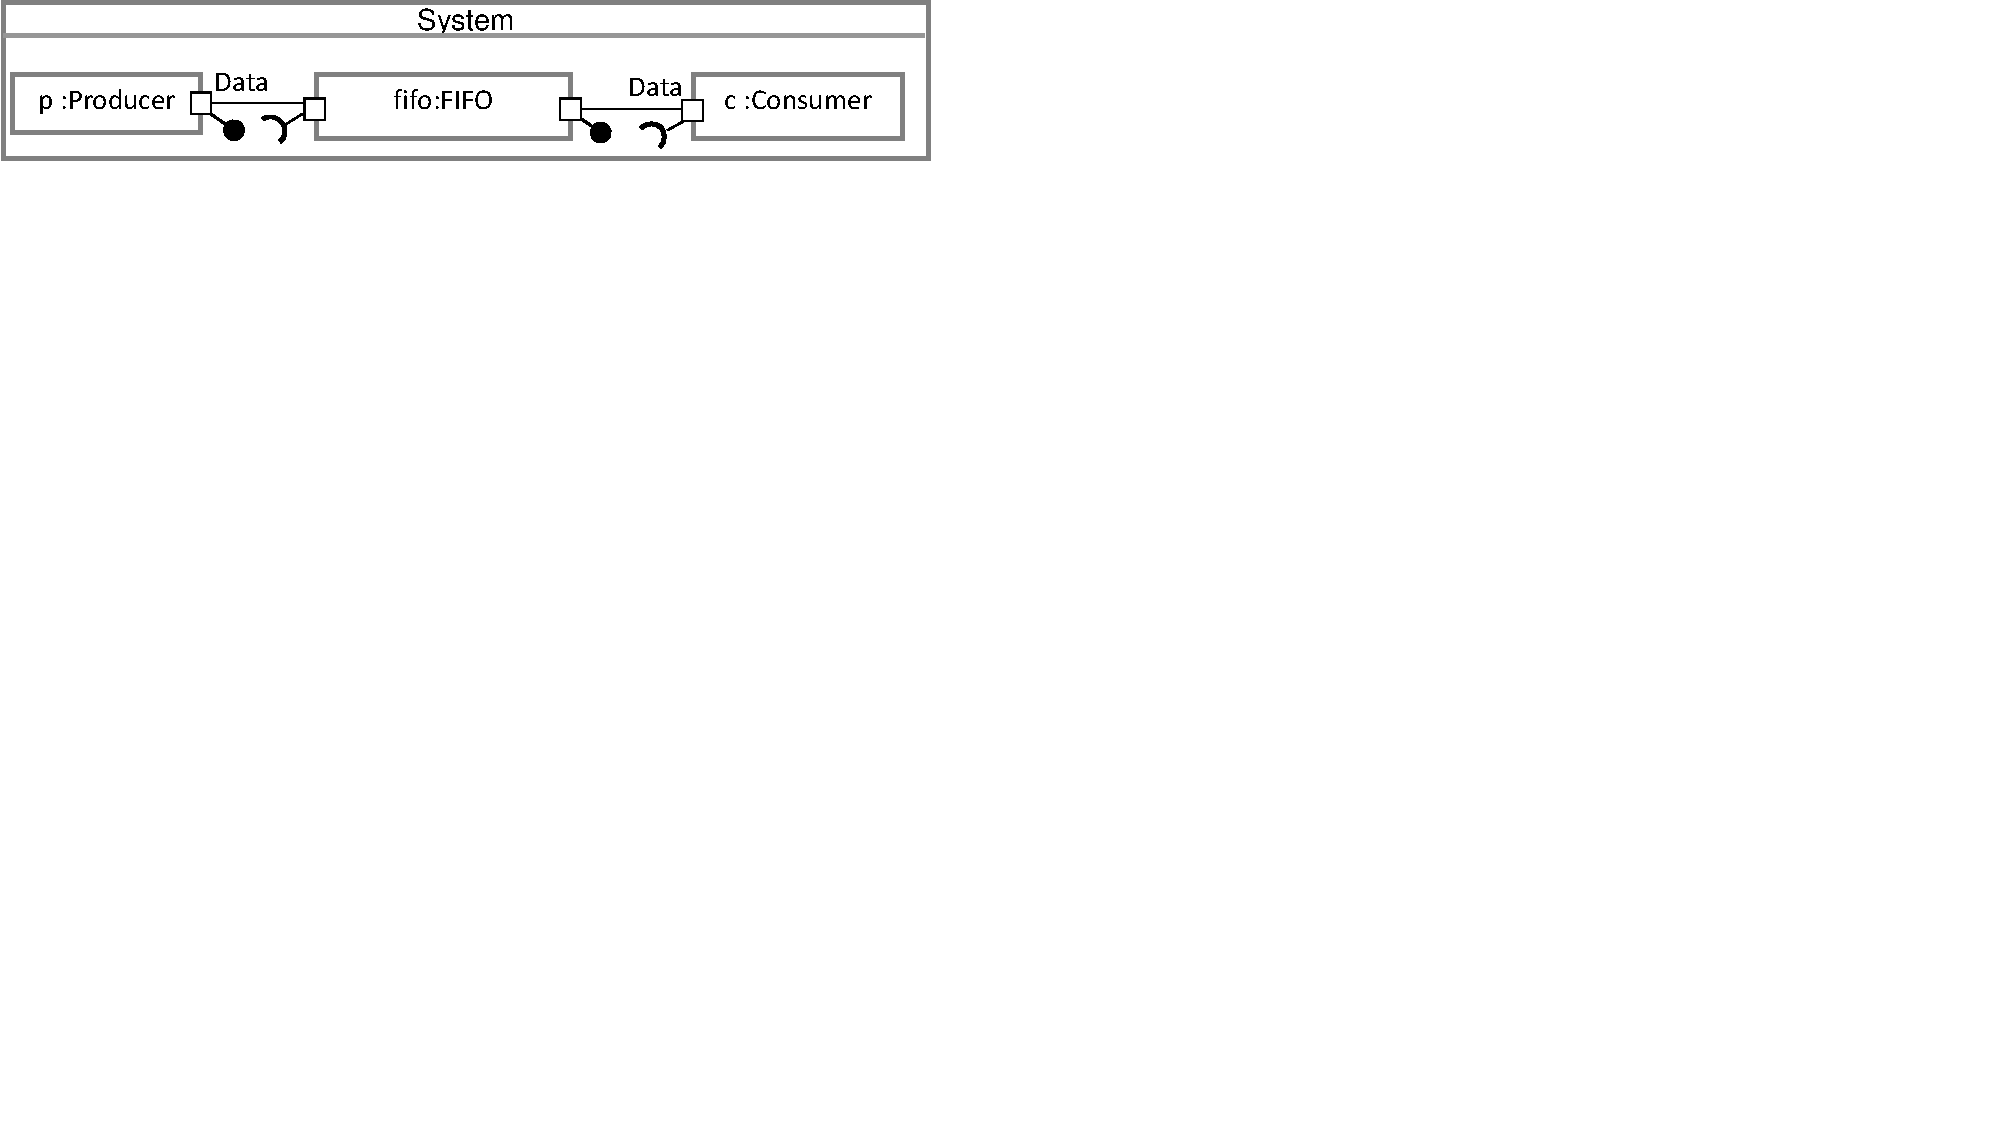
\includegraphics[clip, trim=0cm 16.3cm 17.6cm 0cm, width=\columnwidth]{figures/dataportexample.pdf}
\caption{Component-based architecture example with data port} 
\label{fig:dataportexample}
\end{comment}




Listing \ref{lst:dataport} shows the generated code for the flow port-based producer-consumer example.
The constructs \ti{OutFlowPort} and \ti{InFlowPort} are used.
From an implementation perspective, the producer sends data items to the fifo via the port \ttt{pOutData} by calling \ttt{pOutData.intf->push(item)} (lines 4-6).
Similarly to the service ports, flow ports also have an interface attribute \ti{intf} for writing code to send signals from a component to another component. 
In case the behavior of the receiving component (the fifo, for example) is described by a state machine, the \ttt{push} method will fire a signal event in order for the state machine to handle it. 
The details of signal events are discussed in sub-section \ref{subsec:behavioralconstructs}. 
  

\begin{minipage}{\columnwidth}
	\lstinputlisting[language=C++, caption={Producer-consumer using flow ports}, label=lst:dataport,frame=f]{
		code/dataport.cpp
	}
\end{minipage} 

In the next sub-section, we present our proposed additional programming constructs corresponding to the modeling concepts for the architecture behavior, in particular UML state machine elements.

\subsubsection{Behavioral constructs}
\label{subsec:behavioralconstructs}
%Applying XSeparation to UML State Machines, XSeparation-generated code contains our syntactic sugar of additional constructs for explicitly representing domain-specific concepts of state machines such as states and transitions.
In our approach, UML State Machines are used for modeling the behavior of components. 
Our behavioral programming constructs correspond to UML State Machine concepts at the modeling level. 
These behavioral constructs are grouped into three parts: topology, events, and transition table in the extended code.


\noindent
\tb{Topology:}
A topology contains the constructs to describe the state machine hierarchy.
The root of the topology is specified via the \ttt{StateMachine} as in Fig. \ref{fig:approachexample}.
Other elements such as \ttt{region}, \ttt{state}, and \ttt{pseudo state} are hierarchically defined as state-machine (direct/indirect) sub-elements.
%Each element has a unique name.

State actions such as \ti{entry/exit/doActivity}s are declared within the corresponding state in the extended code as state attributes.
These actions must be implemented as methods in the owning class and have no parameter.
For example, \ttt{Idle} is an initial state. 
The \ttt{SignalChecking} state (lines 36-39) is declared with the state actions, \ti{entryCheck} and \ti{exitCheck}. 
%The latter is specified as following: the entry/exit/doActivity action of a state, if declared within the topology, must be implemented as a method of the component/class. 
The \ti{FIFO} class implements the methods \ttt{entryCheck} and \ttt{exitCheck} (lines 60-61) for the state actions.
%The followings give the syntax of some elements in the generated code and the semantics mapped to the well-defined semantics in the UML specification \cite{OMG2015}.
Programmers can write fine-grained code for these action methods.


Concurrent states with orthogonal regions in the extended code are not shown here due to space limitation. 
Pseudo states can be declared within \ti{Statemachine/states/regions} in the extended code, the syntax is similar to class attribute declarations.
%The type of pseudo state attributes is one of \ttt{\{PseudoEntryPoint, PseudoExitPoint, PseudoInitial, PseudJoin, PseudoFork, PseudoChoice, PseudoJunction, PseudoShallowHistory, PseudoDeepHistory, PseudoTerminate\}}, which correspond to the pseudo states defined in UML State Machine. 
For example, line 49 in Fig. \ref{fig:approachexample} declares the \ti{dataChoice} choice pseudo state mapping to the corresponding pseudo state in the \ti{FIFOMachine} model.   

%\vskip 0.1cm
\noindent
\tb{Events:}
In UML, four event types including \ttt{CallEvent}, \ttt{TimeEvent}, \ttt{SignalEvent}, and \ttt{ChangeEvent} are defined for modeling reactive systems using UML State Machines. 
The semantics of these events are clearly defined in the UML specification and briefly described in the below list.

\begin{itemize}[\footnotesize]
	\itemsep0em
	\item A call event is associated with an operation/method and emitted if the operation is invoked.
	
	\item A signal event is associated with a UML signal type containing data.
	%It is emitted if the class receives an instance of the signal type.
	When a component, whose behavior is described by a UML State Machine, receives a message/signal through its in/inout flow ports, a signal event is automatically emitted and stored in an event queue to be processed by the state machine later.
	
	\item A time event specifies the time of occurrence relative to a starting time, defined as the time when a state with an outgoing transition triggered by the time event is entered.
	The time event is emitted if the state remains active longer than the time of occurrence to trigger the transition.
	%In other words, the state, which is the source vertex of a transition triggered by a time event, will remain active for a maximal amount of time specified by the time event.	

	
	\item A change event has a boolean expression and is fired if the expression's value changes from false to true. 
	%unlike call and signal events, time and change events are automatically fired inside the class.
\end{itemize}

The processing of call events is synchronous meaning that it runs within the thread of the operation caller.
The processing of other events is asynchronous meaning that these events received by a component are stored in an event queue, which is maintained by the component for later processing.
We support all of these events with the same semantics. 

%The code generated by XSeparation for these events has syntax as followings:
\begin{comment}
\begin{itemize}[\footnotesize]
\itemsep0em
\item \ttt{CallEvent} $\rightarrow$ \tb{CallEvent} \tb{(} name\tb{,} op \tb{);}

\item \ttt{TimeEvent} $\rightarrow$ \tb{TimeEvent} \tb{(} name\tb{,} dur \tb{);}

\item \ttt{SignalEvent} $\rightarrow$ \tb{SignalEvent}<sig> name;

\item \ttt{ChangeEvent} $\rightarrow$ \tb{ChangeEvent} \tb{(} name\tb{,} expr \tb{);}
\end{itemize}

Essentially, each field in the syntax carries known semantics defined in the UML specification.
\begin{itemize}[\footnotesize]
\itemsep0em
\item \ttt{name} The unique identifier for an event.

\item \ttt{op} The name of the operation associated with a \ttt{CallEvent} and implemented in the active class. 

\item \ttt{dur} The duration associated with a \ttt{TimeEvent} and specified as millisecond.

\item \ttt{sig} The name of the signal class type (a UML signal is transformed into an object-oriented class) associated with a \ttt{SignalEvent}.
This signal type must be declared as required data of one of ports of the component in \tb{Component structure-prescribed code}.

\item \ttt{expr} The expression associated with a \ttt{ChangeEvent}. This expression is periodically evaluated to check whether its boolean value is changed.
\end{itemize}
\end{comment}

%\ttt{SimpleEvent} is a specialized \ttt{SignalEvent} without specifying an explicit signal.
%It is not explicitly standardized by UML but provided by tools such as QM \cite{qm} for practical reasons. 


%A \ttt{CallEvent} occurs if the method \ttt{method1} in the active class is called.
%\ttt{signal\_event(SE, Sig)}: A \ttt{SignalEvent} occurs if an instance of \ttt{Sig} is sent to the active class using its provided method \ttt{sendSig}.
%\ttt{time\_event(TE5ms, 5)}: A \ttt{TimeEvent} occurs after 5 millisecond from the moment the timer starts by entering some state.


%Call events are synchronous meaning that the processing runs within the thread calling the operation associated with a call event.
%Other events are asynchronous meaning that on receiving these events are stored in an event queue which is maintained at runtime for later processing.                                              
%A time event specifies the time of occurrence relative to a starting time. 
%The latter is specified when a state, which accepts the time event, is entered.
%The time event is emitted if the accepting state, which has at least one outgoing transitions triggered by the event, remains active longer that the relative time of occurrence. 	
%A change event has a boolean expression and is fired if the expression's value changes from false to true. 
%Note that not like call and signal events, time and change events are automatically fired inside the component.


%\vskip 0.1cm
\noindent
\tb{Transition table:}
It describes the mapping of our syntactical constructs to UML transitions at the model level. 
Three kinds of UML transitions, \ttt{external}, \ttt{local}, and \ttt{internal}, are supported but this paper only presents external transitions.
The difference between these kinds is clearly stated in UML and beyond the scope of this paper.
Lines 45-46 in Fig. \ref{fig:approachexample} shows an external transition, which is from \ti{Idle} ti \ti{SignalChecking}, triggered by the \ti{DataPushEvent} call event declared with the state machine, and has \ti{signalCheck} as transition effect.
The \ti{signalCheck} method is implemented within the \ti{FIFO} class owning the state machine, and has the same formal parameters as the \ttt{push} method associated with the call event.

%For example, \ttt{CallEvent(DataPushEvent, push)} at line 23 in Listing \ref{lst:fifostatemachine} specifies that an event is fired whenever the \ttt{push} method, which is implemented by \ttt{FIFO} for the \ttt{IPush} interface provided by the \ttt{pPush} port, is invoked.
For example, line 50 shows a call event, which is emitted whenever there is an invocation of the \ti{push} method of the \ti{FIFO} class. 
The processing of the emitted event activates the transition from \ttt{Idle} to \ttt{SignalChecking}, and executes the \ttt{signalChecking} transition effect method.
The data item returned by the invocation will be checked for validity and further put to the queue or discarded.

%\vskip 0.1cm
\noindent
\tb{Deferred event:}
A state can declare \ttt{deferred events} by introducing attributes typed by our class-like additional construct \ttt{DeferredEvent} and named as event names to be deferred.
A deferred event will not be processed while the state remains active.
The deference of events is used to postpone the processing of some low-priority events while the state machine is in a certain state.
%The deferred events are used for state machine execution to delay the processing of low-priority events.
%The execution semantics of deferred events is that: given a current active state with declared deferred events and an event queue, the deferred events, if in front of the queue, will be moved to a deferred set and pushed back to the front of the queue once a non-deferred event is processed.
%In other words, the deferred events will not be processed while the state remains active.


%Code generated for a signal event has syntax as \tb{SignalEvent}\ttt{<sig> name}, in which \ttt{sig} is the name of the associated signal class (a UML signal is transformed into an object-oriented class).
%The signal type must be declared as required data of one of data ports of the component in \tb{Component structure-prescribed code}.
%Sending of a signal instance to the port might fire an asynchronous signal event for a state machine to handle in case that the containing component behavior of the port is specified via the state machine.
%Due to space limitation, we do not go to details of TimeEvent and ChangeEvent.

%\vskip 0.1cm
%\noindent
%\tb{Configuration:} 
%XSeparation-generated behavior code will be compiled to executable files by using our XSeparation compiler, which is presented in Section \ref{sec:compilation}.
%The executable files run in an asynchronous mode, in which according to UML State Machine, events, except CallEvent, are stored in an event queue at runtime.
 

%\vskip 0.1cm
%\noindent
%\tb{Deferred event:}
%A state can declare \ttt{deferred events} using our additional construct \ttt{DeferredEvent}.
%The deferred events are used for state machine execution to delay the processing of low-priority events when a certain state is active.
%The execution semantics of deferred events is that: given a current active state with declared deferred events and an event queue, the deferred events, if in front of the queue, will be moved to a deferred set and pushed back to the front of the queue once a non-deferred event is processed.
%In other words, the deferred events will not be processed while the state remains active.


\section{XSeparation Compiler}
\label{sec:compilation}
%XSeparation generates object-oriented code containing additional constructs for bidirectional traceability. Hence, a compilation process is needed to transform the XSeparation-generated code into machine code.
This section presents the architecture of the XSeparation compiler. %to transform the XSeparation-generated code into machine code.
\begin{figure}
	\centering
	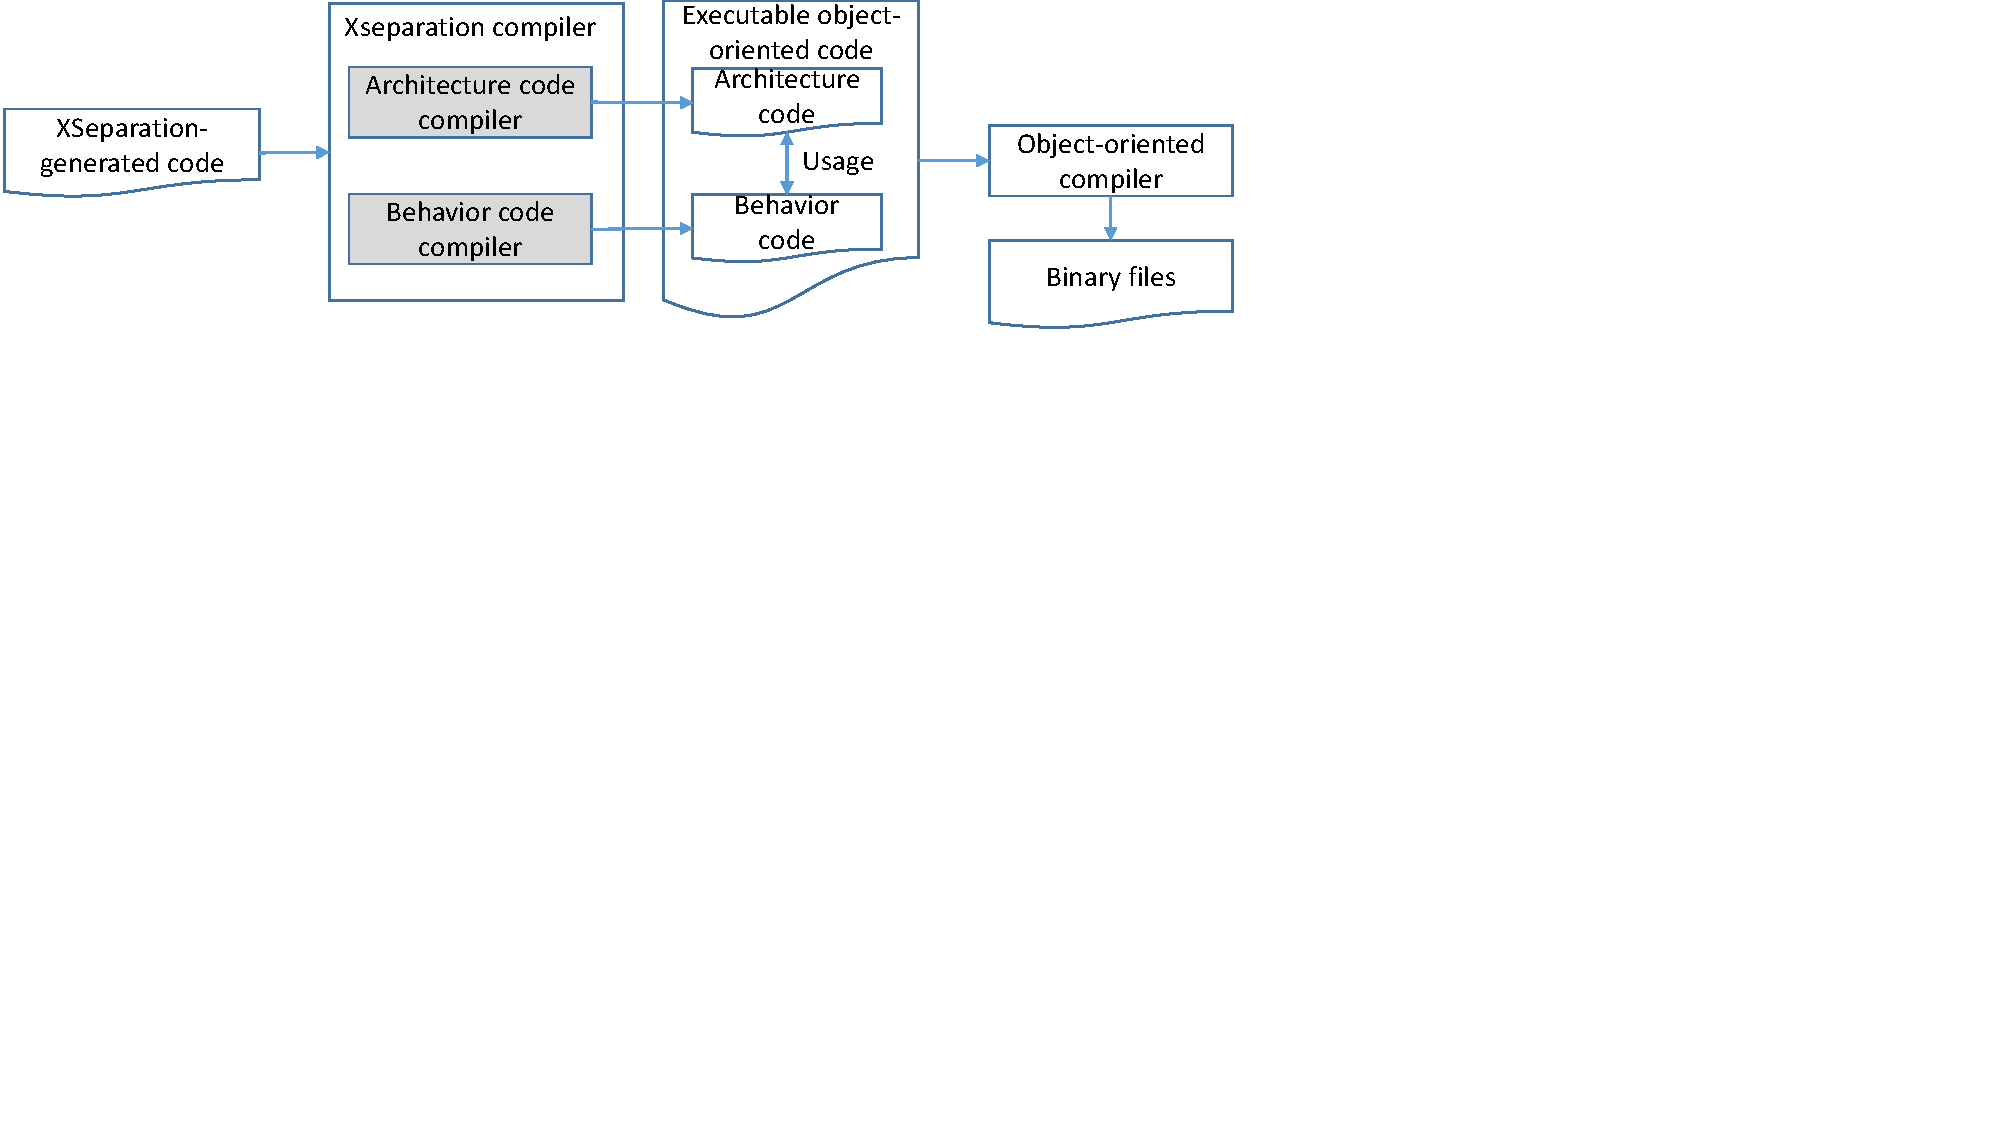
\includegraphics[clip, trim=0cm 13.3cm 12.8cm 0cm, width=\columnwidth]{figures/compilerarchitecture.pdf}
	\caption{XSeparation compiler's architecture} 
	\label{fig:compilerarchitecture}
\end{figure}
Fig. \ref{fig:compilerarchitecture} shows the compilation process, which takes as input the XSeparation-generated code, and produces the binary files by three two steps: \textcircled{1} generation of executable object-oriented code by the XSeparation compiler from XSeparation-generated code; \textcircled{2} production of binary files from the executable code by using object-oriented compilers such as GCC for C++ and Javac for Java.

The XSeparation compiler consists of two grayed sub-modules: \tb{Structure code compiler}, which takes as input the \tb{Component structure-prescribed code}, \tb{User-filled skeleton code}, and \tb{Component structure-provided implementation code} parts to produce \tb{Structure code}, while \tb{Behavior code compiler} takes as input the other parts to generate \tb{Behavior code}. 



\vskip 0.1cm
\noindent
\tb{Structure code compiler:}
A verification is firstly executed to check the well-formedness of components and ports.
We basically verify three port rules: (1) every port with a required interface or provided data must be bound to another port; (2) if two ports are connected by a assemble connector, the provided interface/data of one port must identical to or an extension of the required interface/data of the other port; and (3) if the connector is delegate, the provided interface/data of one port must identical to or an extension of the provided interface/port of the other port; 

Once the rules are verified, executable code can be generated. 
Listing \ref{lst:archcodecompiler} shows a \tb{Structure code} segment generated from the \ttt{System} example using ports with interfaces.
Each port is generated to a pointer attribute (lines 12 and 15) while each part to an object attribute (lines 3,4,5).
A configuration is transformed into a method named \ttt{configuration}.
When a method is called through a port as in Listing \ref{lst:producerinteraction}, for example \ttt{push} through the \ttt{pPush} port, the corresponding method implemented in FIFO is invoked. 

\begin{minipage}{\columnwidth}
	\lstinputlisting[language=C++, caption={Executable code generated by XSeparation compiler for the structure of \ttt{System}}, label=lst:archcodecompiler,frame=f]{code/archcodecompiler.cpp}
\end{minipage} 

\vskip 0.1cm
\noindent
\tb{Behavior code compiler:}
It generates executable code from the \tb{Behavior-prescribed code} and \tb{State machine action code} similarly to code generation approaches from UML State Machines in MDE tools such as Rhapsody and Sinelabore \cite{sinelabore}.
However, only a subset of UML State Machine concepts is supported by these tools, e.g. Rhapsody does not support junctions, and truly concurrent execution of orthogonal regions
\cite{ibmdiff} (see \cite{specification_uml_2007} for more detail) and the support for pseudo states such as history, choice and junction is poor \cite{EA, sinelabore}. 
%The concurrency of the orthogonal regions is often implemented sequentially \cite{Badreddin2014}. 
%In addition, there are other issues such as event processing speed, executable file size, and UML semantic-conformance defined by a recent work on the Precise Semantics of State Machine (PSSM) \cite{OMG2015}.
XSeparation compiler supports full features of state machines.
XSeparation compiler has following unique features:

\begin{itemize}[\footnotesize]
	\item \tb{Completeness:} XSeparation compiler supports all state machine vertexes and transitions including all pseudo states and transition kinds. 
	Hence, XSeparation compiler improves flexibility of using state machines to express architecture behavior.
	For the moment, the only issue with the compiler is that it cannot deal with transitions from an entry point to an exit point.
	
	\item \tb{Event support:} XSeparation compiler utilizes four UML event types and deferred events, which are able to express synchronous and asynchronous behaviors and exchange data between components.
	
	\item \tb{UML-conformance:} A recent specification formalizing the precise semantics of UML State Machine is under standardization of OMG.
	It defines a test suite with 66 test cases for certifying the conformance of runtime execution of code generated from UML State Machines.
	We have experimented XSeparation compiler with the test suite.
	The traced execution results of 62/66 test cases comply with the standard and are a good hint that the execution is semantically correct.
	Due to space limitation, the details of patterns and evaluation for state machine code generation semantics are not presented in this paper.
	
	\item \tb{State machine configuration:} XSeparation allows to configure the event queue size and periodic time for evaluation of change events.
	
	\item \tb{Event API:} Generated code in XSeparation compiler provides APIs for environment code to invoke operations or send data signals through component ports.
	The invocations and sending will automatically fire events for state machines to process.
\end{itemize}


In the next section, XSeparation will be implemented as an extension of the Papyrus modeling tool and evaluated by developing a case study of software application for LEGO.